\section{Sensorer} \label{sec:sensorer}
I det tiltænkte system benyttes forskellige sensorer, hvorfra systemet skal agere. Herunder benyttes elektroder til opsamling af EMG-signaler, hvilket yderligere vil passere en EMG-forstærker, Muscle Sensor V3. %Herudover vil accelerometeret ADXL335Z benyttes til måling af accerlerationskræfter.

\subsection{Elektromyografi}
Elektromyografi (EMG) er en måling af muskelaktivitet gennem elektriske potentialer. 
EMG-forstærkeren er designet til at kunne anvendes direkte med en mikrocontroller. Signalets output er herved ikke et råt EMG-signal, men et forstærket, ensrettet samt udglattet signal \citep{advancertech2013}. Udglatningen består af et aktivt lavpasfilter, hvor udregningen af knækfrekvensen ses i \autoref{eq:lavcutfre}. 

\begin{equation}\label{eq:lavcutfre}
f_c = \frac{1}{2 \pi C R} = \frac{1}{2 \pi*1*10^{-6}F*80,6*10^3\Omega} = 1,94~Hz
\end{equation}

Et illustration af hvordan EMG-forstærkeren behandler et målt signal ses af \autoref{fig:sinussignal}.

\begin{figure}[H]
\centering
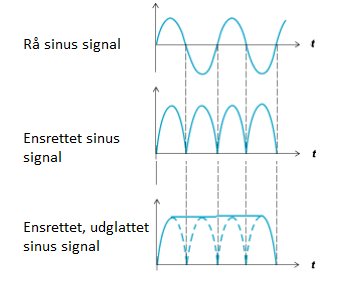
\includegraphics[width=0.8\textwidth]{figures/sinussignal.png}
\caption{Tre sinus signaler. Henholdsvis et råt sinus signal, ensrettet sinus signal og ensrettet samt udglattet sinus signal \citep{advancertech2013}.}
\label{fig:sinussignal}
\end{figure}

Muskelsensoren V3 har en minimum spændingsforsyning på $\pm$ 3 V samt en maksimal spændingsforsyning på $\pm$ 30 V. Herudover er der mulighed for at justere gain fra 0,002 gange - 20,700 gange \citep{advancertech2013}.

%Synes ikke det passer ind her? Er det ikke meningen dette skal være mere overordnet, og så specificerer vi os senere til hvordan vi vil måle, sådan til vores forsøg?
%Den ene elektrode placeres over enten rectus femoris eller vastus intermedius (sidder under rectus femoris) og den anden elektrode placeres over biceps femoris. Reference elektroden placeres ved??.. 



%\subsection{Accelerometer}
%Et accelerometer er en elektromekanisk enhed, som både kan måle statiske eller dynamiske accerlerationskræfter. De statiske kræfter kan være tyngdekraften, hvortil det er muligt at bestemme orienteringen af accelerometeret i forhold til jorden. De dynamiske kræfter såsom bevægelse, stød og vibrationer, gør det muligt at analysere accelerometeres bevægelse samt hastighed. 
%ADXL335Z er et 3-aksialt accelerometer, som har et arbejdsområde på minimum $\pm$ 3 g. Hertil arbejdes der ved dette accelerometer med analoge output signaler proportionelle med accelerationen \citep{analogdevices2010}. 

%\textbf{Tilføj noget om sensitivitet og evt. illustration af g-påvirking og udregning af vinkel skal tilføjes hertil.}

%Støj kan reduceres ved at placere en 0.1 mikro f capacitor i nærheden, det er dog nødvendigt at tilføje mere, hvis der er 50 KHz støj, da det vil kunne resultere i fejl i accelerations målingen. Støjens tæthed vil forminskes i takt med at forsyningsspændingen forøges.
%Fase sensitiv demodulation teknikker er anvendt for at bestemme magnituden samt accelerationens retning. Demodulator outputtet er forstærket og bragt igennem en 32 k ohm modstand. – noget med det forebygger aliasing 
%  - Jeg ser dette som 'ligegyldigt' nu, da det handler om kondensator og støj. Kan ikke se hvorfor det skal bruges (endnu) måske skal det bruges efter vi har lavet pilotforsøg, hvis der viser sig meget støj





